\documentclass[10pt,a4paper]{article}

\usepackage{polski} 
\usepackage[utf8]{inputenc}
\usepackage[comma]{natbib}
\usepackage[top=2.5cm, bottom=2.5cm, left=2.5cm, right=2.5cm]{geometry}
\usepackage{amsmath,bm,amsfonts,amssymb}
\usepackage{wasysym}
\usepackage{xcolor}
\usepackage{graphicx}
\DeclareGraphicsExtensions{.pdf,.eps,.png,.jpg}
\usepackage{float}           
\usepackage{subfloat}          
\usepackage{caption}             
\usepackage{subcaption}
\usepackage{array}
\usepackage{multicol}   % \multicolumn{num_cols}{alignment}{contents}
\usepackage{multirow}   % \multirow{''num_rows''}{''width''}{''contents''} {* for the width means the content's natural width}
\usepackage{booktabs}           % tabele (toprule/midrule/bottomrule)

\newcommand{\logoGIK}{WGiK-znak.png}
\newcommand{\authorName}{Hanna Łempcika  \\ grupa 2a, Numer Indeksu: 291360}

\newcommand{\titeReport}{Wyznaczenie punktu przeciecia dwóch odcinków} % <<< insert short title in the food
\newcommand{\titleLecture}{Informatyka Geodezyjna \\ sem. IV, ćwiczenia, rok akad. 2018-2019} % <<< insert title of presentation
\newcommand{\kind}{report}
\newcommand{\mymail}{\href{mail to:} {hania.lempicka@wp.pl}}
\newcommand{\supervisor}{....}
\newcommand{\gikweb}{\href{www.gik.pw.edu.pl}{www.gik.pw.edu.pl}}
\newcommand{\institut}{Katedra Geodezji Wyższej i Astronomii}
\newcommand{\faculty}{Wydział Geodezji i Kartografii}
\newcommand{\university}{Politechnika Warszawska}
\newcommand{\city}{Warszawa}
\newcommand{\thisyear}{2019}
%\date{}
% PDF METADATA
\pdfinfo
{
	/Title       (GIK PW)
	/Creator     (TeX)
	/Author      (Hanna Łempicka)
}


% ------------------------- POCZATEK DOKUMENTU -------------------
\begin{document}
	% -----------------------------------------------------------------------------------------
	% ----------------------------  Title page
	% -----------------------------------------------------------------------------------------
	\begin{center} 
		\rule{\textwidth}{.5pt} \\
		\vspace{1.0cm}
		\includegraphics[width=.4\paperwidth]{\logoGIK}
		\vspace{0.5cm} \\
		\Large \textsc{\titeReport}
		\vspace{0.5cm} \\  
		\large \textsc{\titleLecture}
		\vspace{0.5cm}\\
		\textsc{\authorName}  \\
		\textsc{\faculty}, \textsc{\university}  \\ 
		\city, \thisyear
	\end{center} 
	\rule{\textwidth}{1.5pt}
	
	% -----------------------------------------------------------------------------------------
	% ----------------------------  Table of content
	% -----------------------------------------------------------------------------------------
	\tableofcontents 								% wyświetla spis treści
	%\addcontentsline{to}{chapter}{Spis treści} 	% dodaje pozycję do spisu treści
	
	%
	%

\newpage
\section{Sposób rozwiązania problemu}

\subsection{Wyzanczenie punktu przecięcia}
Punkt przecięcia wyznaczyłam za pomocą metody z wyznacznikami t1 i t2, podaną na zajęciach. Definicja została zapisana w pliku PunktPrzeciecia.py.

\subsection{Aplikacja}
Wyniki funkcji przedstawiłam w wygodniej dla użytkownika formie - aplikacji GUI. Używałam do tego PyQt5. W widgetcie wykorzystałam Label (do opisów), Edit (do wyświetlania wyników lub wpisywania danych), button (do przeliczeń) oraz figure (do wyświetlenia wykresu). 
\\
Funckje:
\begin{itemize}
	\item SprawdzLiczbe - funkcja do sprawdzania czy wpisana przez użytkownika dana jest liczbą
	\item czysc - funckja która czyści wszystkie wymienione w niej pola 
	\item zmienKolor, zmienKolor2 - Zmiana koloru lini na wykresie
	\item oblicz - Ślepa funkcja stworzona po to by defincja rysuj mogła mieć trzy zmienne 
	\item rysuj - W tej defincji używam wszystkich pozostałych. Na początku sprawdzam czy podane dane są prawidłowe, następnie sczytuję je i wykorzystuję je do obliczenia punktu przecięcia (z wykorzystaniem definicji PunktPrzeciecia). Następnie rysuję wykres na którym będzie: linie AB i CD, punkt P oraz przedłużenia lini AB i CD jeśli punkt nie leży na nich. Ta właśnie funkcja wyświetla wyniki czyli: współrzędne punktu oraz położenie punktu. Dodatkowo wykorzystując funcję liczenia azymutu z pliku azymut.py liczy azymut dla obydwu lini oraz wyświetla jego wartość i rysuje jego szkic na wykresie. 
\end{itemize}

\section{Instrukacja obsługi aplikacji}
\begin{figure}[h]
	\centering
	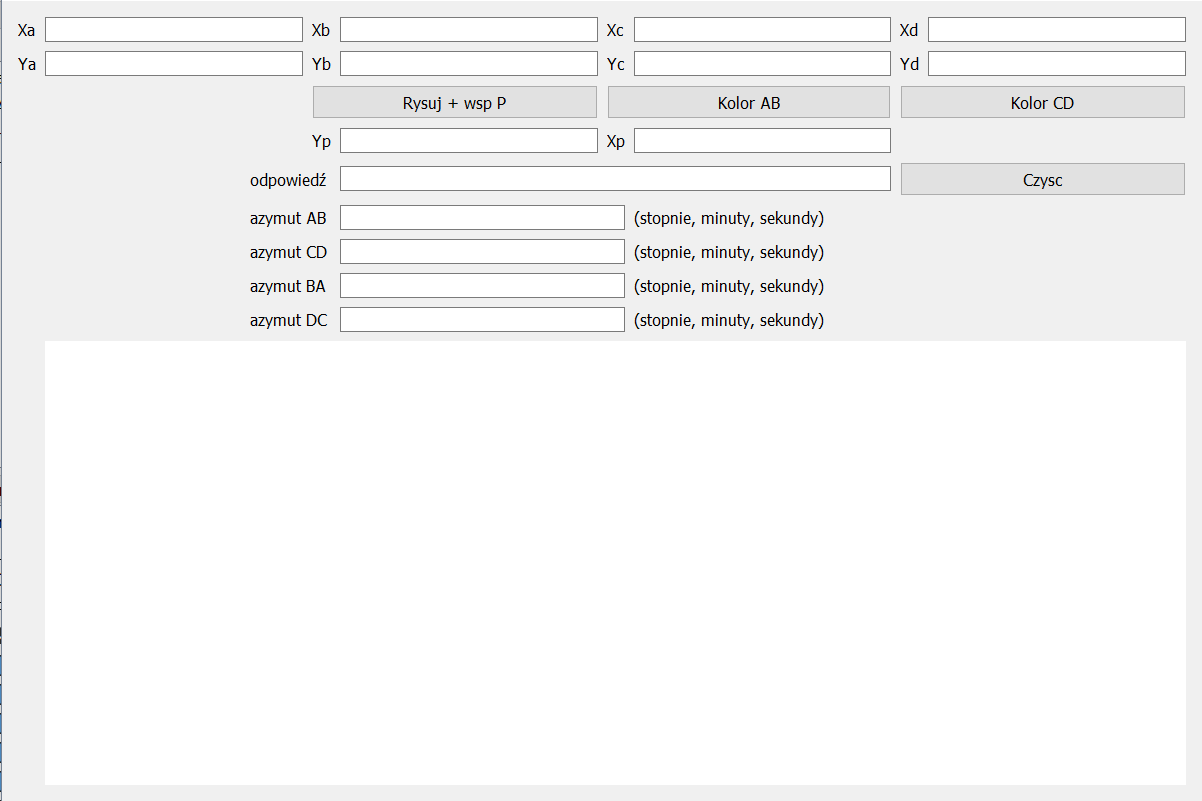
\includegraphics[width=10cm]{apka.PNG}
\end{figure}
W miejscach opisanych Xa, Ya, Xb, Yb, Xc, Yc, Xd, Yd należy wpisać współrzędne odcinków dla których chcemy wyznaczyć punkt przecięcia. Następnie należy należy przycisnąć przycisk "Rysuj + wsp P". Spowoduje to policzenie współrzędnych punktu przecięcia, azymutów obu odcinków oraz narysuje wykres. Dodatkowo można przyciskiem Kolor AB lub kolor CD zmienić kolor lini albo przycisnąć Czysc by wyczyścić wszystkie pola. 

\section{Repositorie}
Link do repository - https://github.com/HannaLempicka/Projekt1$\_$InfGeo2.git

\end{document}